% begin module one-to-one-def
\begin{frame}
\frametitle{One-to-one Functions}
\begin{definition}[One-to-one Function]
A function $f$ is a one-to-one function if it never takes on the same value twice; that is,
\[
f(x_1) \neq f(x_2) \ \text{whenever }  \ x_1 \neq x_2 .
\]
\end{definition}
\begin{columns}[c]
\column{.5\textwidth}
\psset{xunit=1.3cm, yunit=1.3cm}
\begin{pspicture}(-5, -5)(5,5) 
\psframe*[linecolor=white](-5,-5)(5,5) 
\psaxes[ticks=none, labels=none]{<->}(0,0)(-0.5,-0.5)(3.9,3)
%Function formula: -1/2*((-17/10+x)^{2})+9/5 
\psplot[linecolor=red, plotpoints=1000]{-0.5}{3.9}{1.8 x -1.7 add 2 exp -0.5 mul add }
\rput[b](1.7, 1.9) {\footnotesize $y=f(x)$}

\psFullDot{0.7}{1.3}
\rput[br](0.6, 1.4) {\footnotesize $(x_1, f(x_1))$}
\psFullDot{2.7}{1.3}
\rput[bl](2.8, 1.4) {\footnotesize $(x_2, f(x_2))$}

\psline(-0.5, 1.3)(3, 1.3)
\rput[t](1.7, 1.2) {\footnotesize $y=f(x_1)=f(x_2)$}

\psline(0.7, -0.1)(0.7, 0.1)
\rput[t](0.7, -0.2){\footnotesize $x_1$}
\psline(2.7, -0.1)(2.7, 0.1)
\rput[t](2.7, -0.2){\footnotesize $x_2$}

\end{pspicture} 
%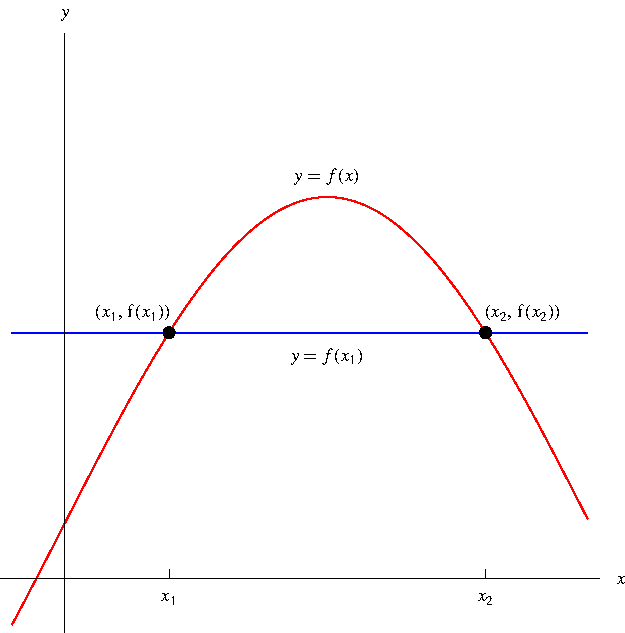
\includegraphics[height=5cm]{inverse-functions/pictures/07-01-1-1def.pdf}%
%
\column{.5\textwidth}
$\leftarrow$ This function is not one-to-one.
\end{columns}
\end{frame}
% end module one-to-one-def
